\chapter{Weryfikacja i walidacja}
\label{ch:06}

Z uwagi na implementację programu na karcie graficznej jako jednostkę cieniującą fragmentów, weryfikacja poprawności jego działania jest znacznie utrudniona. Programując w języku GLSL brak jest możliwości zastosowania testów jednostkowych, co spowodowało, że testowanie sprowadzało się do metody prób i błędów. Przeprowadzono porówynywania różnych technik i wzorów by uzyskać pożądany efekt. Ewentualne niepoprawne obliczenia są często niewidoczne mimo wydawało by się poprawnego działania. Jednym z takich problemów było obliczanie wektorów normalnych powierzchni, co spowodowane było niepoprawnym zastosowaniem wzoru. Błąd ten ujawnił się dopiero po implementacji cieni, gdy oświetlone powierzchnie były przyciemnione, sprawiały wrażenie, że były odwrócone od źródła światła. Defekt ten przedstawia rysunek \ref{fig:normals}.

\begin{figure}[H]
\centering
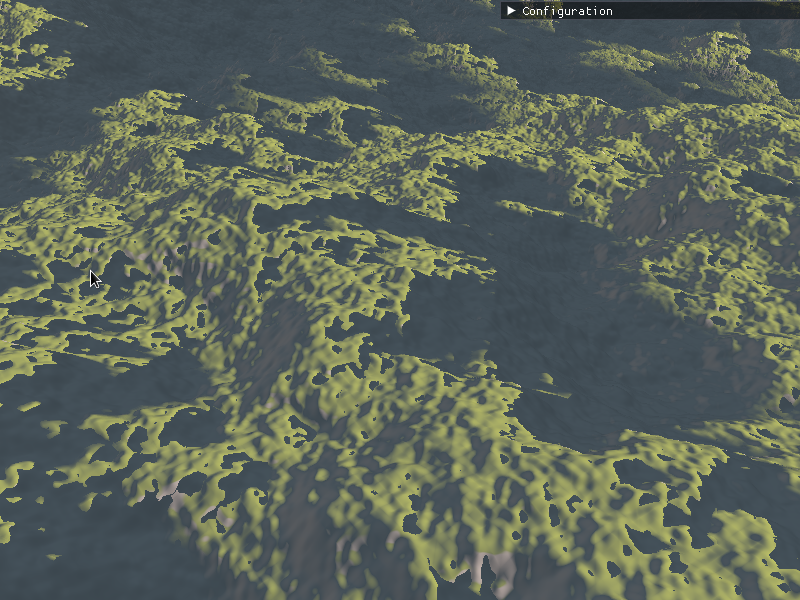
\includegraphics[width=1\textwidth]{./graf/norm.png}
\caption{Niepoprawne obliczanie wektorów normalnych.}
\label{fig:normals}
\end{figure}

%% \begin{itemize}
%% \item sposób testowania w ramach pracy (np. odniesienie do modelu V)
%% \item organizacja eksperymentów
%% \item przypadki testowe zakres testowania (pełny/niepełny)
%% \item wykryte i usunięte błędy
%% \item opcjonalnie wyniki badań eksperymentalnych
%% \end{itemize}

%% \begin{table}
%% \centering
%% \caption{Nagłówek tabeli jest nad tabelą.}
%% \label{id:tab:wyniki}
%% \begin{tabular}{rrrrrrrr}
%% \toprule
%% 	         &                                     \multicolumn{7}{c}{metoda}                                      \\
%% 	         \cmidrule{2-8}
%% 	         &         &         &        \multicolumn{3}{c}{alg. 3}        & \multicolumn{2}{c}{alg. 4, $\gamma = 2$} \\
%% 	         \cmidrule(r){4-6}\cmidrule(r){7-8}
%% 	$\zeta$ &     alg. 1 &   alg. 2 & $\alpha= 1.5$ & $\alpha= 2$ & $\alpha= 3$ &   $\beta = 0.1$  &   $\beta = -0.1$ \\
%% \midrule
%% 	       0 &  8.3250 & 1.45305 &       7.5791 &    14.8517 &    20.0028 & 1.16396 &                       1.1365 \\
%% 	       5 &  0.6111 & 2.27126 &       6.9952 &    13.8560 &    18.6064 & 1.18659 &                       1.1630 \\
%% 	      10 & 11.6126 & 2.69218 &       6.2520 &    12.5202 &    16.8278 & 1.23180 &                       1.2045 \\
%% 	      15 &  0.5665 & 2.95046 &       5.7753 &    11.4588 &    15.4837 & 1.25131 &                       1.2614 \\
%% 	      20 & 15.8728 & 3.07225 &       5.3071 &    10.3935 &    13.8738 & 1.25307 &                       1.2217 \\
%% 	      25 &  0.9791 & 3.19034 &       5.4575 &     9.9533 &    13.0721 & 1.27104 &                       1.2640 \\
%% 	      30 &  2.0228 & 3.27474 &       5.7461 &     9.7164 &    12.2637 & 1.33404 &                       1.3209 \\
%% 	      35 & 13.4210 & 3.36086 &       6.6735 &    10.0442 &    12.0270 & 1.35385 &                       1.3059 \\
%% 	      40 & 13.2226 & 3.36420 &       7.7248 &    10.4495 &    12.0379 & 1.34919 &                       1.2768 \\
%% 	      45 & 12.8445 & 3.47436 &       8.5539 &    10.8552 &    12.2773 & 1.42303 &                       1.4362 \\
%% 	      50 & 12.9245 & 3.58228 &       9.2702 &    11.2183 &    12.3990 & 1.40922 &                       1.3724 \\
%% \bottomrule
%% \end{tabular}
%% \end{table}
